\documentclass[titlepage, letterpaper, fleqn]{article}
\usepackage[utf8]{inputenc}
\usepackage{fancyhdr} % fancy headers, of course!
\usepackage{amsmath} % what do you think?
\usepackage{amsthm} % theorems!
\usepackage{extramarks} % more cute things
\usepackage{enumitem} % i'm not sure...
\usepackage{multicol} % multicolumn...?
\usepackage{amssymb} % more symbols
\usepackage{MnSymbol} % moar symbols?
\usepackage{booktabs} % cool looking tables
\usepackage{tikz} %venn and shizzle
\usepackage{mathrsfs} %math script for calligraphic scripting, I GUESS
\usepackage{listings}
\usepackage{mathtools}
\usepackage[spanish, mexico]{babel}

\topmargin=-0.45in
\evensidemargin=0in
\oddsidemargin=0in
\textwidth=6.5in
\textheight=9.0in
\headsep=0.25in


%
% You should change this things~
%

\newcommand{\mahteacher}{Dr. Ernesto Rodríguez Leal}
\newcommand{\mahclass}{Robótica}
\newcommand{\mahtitle}{Cinemática Directa}
\newcommand{\mahdate}{\today}

\newcommand{\spacepls}{\vspace{5mm}}
\renewcommand\qedsymbol{\(\blacksquare\)}
\renewcommand{\ttdefault}{pcr} %so we can get both bold and tt fonts

\newcommand{\bigO}{\mathcal{O}} %you should be inside a math environment
\let\bs\mathbf

%
% Header markings
%

\pagestyle{fancy}
\lhead{}
\chead{}
\rhead{}
\lfoot{}
\rfoot{}


\renewcommand\headrulewidth{0.4pt}
\renewcommand\footrulewidth{0.4pt}

\setlength\parindent{0pt}
\setlength\parskip{0.5pt}


%
% Create Problem Sections (stolen directly from jdavis/latex-homework-template @ github!)
%

\newcommand{\enterProblemHeader}[1]{
\nobreak\extramarks{}{Problem \arabic{#1} continued on next page\ldots}\nobreak{}
\nobreak\extramarks{Problem \arabic{#1} (continued)}{Problem \arabic{#1} continued on next page\ldots}\nobreak{}
}

\newcommand{\exitProblemHeader}[1]{
\nobreak\extramarks{Problem \arabic{#1} (continued)}{Problem \arabic{#1} continued on next page\ldots}\nobreak{}
\stepcounter{#1}
\nobreak\extramarks{Problem \arabic{#1}}{}\nobreak{}
}

\setcounter{secnumdepth}{0}
\newcounter{partCounter}
\newcounter{homeworkProblemCounter}
\setcounter{homeworkProblemCounter}{1}
\nobreak\extramarks{Exercise \arabic{homeworkProblemCounter}}{}\nobreak{}

%Solution Environment
% \newenvironment{solution}
% {\renewcommand\qedsymbol{$\square$}\begin{proof}[Solution]}
% {\end{proof}}

% Alias for the Solution section header
\newcommand{\solution}{\textbf{\Large Solution}}

%Alias for the new step section
\newcommand{\steppy}[1]{\textbf{\large #1}}

%
% Homework Problem Environment
%
% This environment takes an optional argument. When given, it will adjust the
% problem counter. This is useful for when the problems given for your
% assignment aren't sequential. See the last 3 problems of this template for an
% example.
%
\newenvironment{homeworkProblem}[1][-1]{
\ifnum#1>0
\setcounter{homeworkProblemCounter}{#1}
\fi
\section{Problem \arabic{homeworkProblemCounter}}
\setcounter{partCounter}{1}
\enterProblemHeader{homeworkProblemCounter}
}{
\exitProblemHeader{homeworkProblemCounter}
}

%
% My actual info
%

\title{
\vspace{1in}
\textbf{Tecnológico de Monterrey} \\
\vspace{0.5in}
\textmd{\mahclass} \\
\large{\textit{\mahteacher}} \\
\vspace{0.5in}
\textsc{\mahtitle}\\
\author{00783957 -- Alicia del Río \\
\and 00952040 -- Cristina Aparicio \\
\and 00822833 -- Guillermo Sotelo \\
\and 00809576 -- Sergio Sedas \\
\and 01170065 -- Xavier Sánchez}
\date{\mahdate}
}

\begin{document}

\begin{titlepage}
\maketitle
\end{titlepage}

%
% Actual document starts here~
%

\section{Cinemática Directa} % (fold)
\label{sec:forward}

Esta sección describe las ecuaciones del análisis de cinemática directa asumiendo que tenemos el diagrama justo como en~\cite{Rodriguez-Leal2011}, muy parecido al diagrama siguiente.

\begin{figure}[htbp]
    \centering
    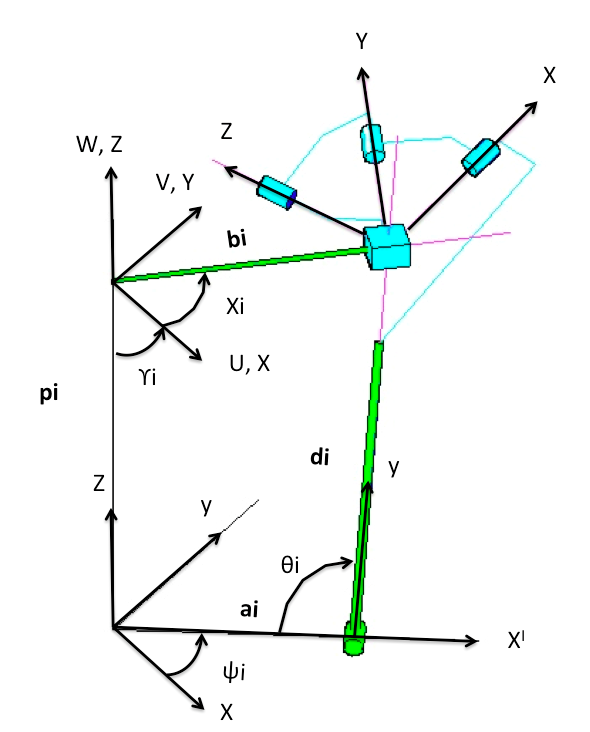
\includegraphics[width=0.5\textwidth]{02-diagram}
    \caption{Diagrama para la $i$-ésima articulación}
    \label{fig:label}
\end{figure}

La sección está dividida en subsecciones dependiendo del tipo de ecuaciones que se trate.

\subsection{Punto de Fermat-Torricelli}
\label{subsec:fermat-torricelli}

El punto de Fermat-Torricelli de un triángulo es un punto en el que la suma de las distancias a los vértices del triángulo es mínima.
Este punto representa el centro de la plataforma del efector final, es decir, el punto $p$ de la Ecuación~\ref{eq:loop_closure}.

Para hallar este punto se utilizó un enfoque algebraico, el cual es ampliamente desarrollado en~\cite{Palacios-Velez2015}.
El enfoque de Palacios-Vélez et al. encuentra los componentes $x,$ y $ y$ del punto de Fermat-Torricelli utilizando las siguientes ecuaciones:

\begin{equation}
    \label{eq:fermat_x}
    xFermat = \frac{xb(\sqrt{3}xc + yc)(xb + xc + \sqrt{3} yc)}{2\sqrt{3}(xb^2 - xb xc + xc^2 + yc^2 + \sqrt{3} xb yc)}
\end{equation}

\begin{equation}
    \label{eq:fermat_y}
    yFermat = \frac{xb(\sqrt{3}xc + yc)(\sqrt{3}(xb - xc) + yc)}{2\sqrt{3}(xb^2 - xb xc + xc^2 + yc^2 + \sqrt{3} xb yc)}
\end{equation}

Donde $xa, xb, xc$ representan los componentes $x$ de los vértices $A, B, C$ respectivamente.
De manera análoga, $yc$ representa el componente $y$ del vértice $C$.

Tras obtener las coordenadas del punto en un plano de dos dimensiones, se procedió a convertir el plano a tres dimensiones para poder encontrar la distancia con respecto al origen.

PENDIENTE

\subsection{Lazo cerrado} % (fold)
\label{subsec:loop_closure}

% subsection loop-closure (end)

\begin{equation}
    \label{eq:loop_closure}
    p+b_i = a_i + d_i
\end{equation}

\begin{equation}
    \label{eq:p_vector}
    \bs{p} = [p_x,p_y,p_z]^T
\end{equation}

\begin{equation}
    \label{eq:a_vector}
    \bs{a}_i = \bs{R}(Z,\psi_i) \cdot [a,0,0]^T
\end{equation}

\begin{equation}
    \label{eq:b_vector}
    \bs{b}_i = \bs{R}(Z,\chi_i)\cdot \bs{R}(Z, \gamma_i) \cdot \bs{R}(Y, \beta_i) \cdot [0, b_i, 0]^T
\end{equation}

\begin{equation}
    \label{eq:d_vector}
    \bs{d}_i = \bs{R}(Z,\psi_i) \cdot \bs{R}(\prescript{I}{}{Z},\phi) \cdot \bs{R}(\prescript{II}{}{X}, \theta_{i1})[0,d,0]^T
\end{equation}

\subsection{Matrices de rotación} % (fold)
\label{subsec:rotations}

\begin{equation}
    \label{eq:rot_Z_psi}
    \bs{R}(Z,\psi_i) =
    \begin{bmatrix}
        \cos\psi_i & -\sin\psi_i & 0 \\
        \sin\psi_i & \cos\psi_i & 0 \\
        0 & 0 & 1
    \end{bmatrix}
\end{equation}

\begin{equation}
    \label{eq:rot_Z_phi}
    \bs{R}(Z,\phi_i) =
    \begin{bmatrix}
        \cos\phi_i & -\sin\phi_i & 0 \\
        \sin\phi_i & \cos\phi_i & 0 \\
        0 & 0 & 1
    \end{bmatrix}
\end{equation}

\begin{equation}
    \label{eq:rot_X_theta}
    \bs{R}(X,\theta_{i1}) =
    \begin{bmatrix}
        1 & 0 & 0 \\
        0 & \cos\theta_{i1} & -\sin\theta_{i1} \\
        0 & \sin\theta_{i1} & \cos\theta_{i1}
    \end{bmatrix}
\end{equation}

\begin{equation}
    \label{eq:rot_Z_chi}
    \bs{R}(Z,\chi_i) =
    \begin{bmatrix}
    \cos\chi_i & -\sin\chi_i & 0 \\
    \sin\chi_i & \cos\chi_i & 0 \\
    0 & 0 & 1
    \end{bmatrix}
\end{equation}

\begin{equation}
    \label{eq:rot_Z_gamma}
    \bs{R}(Z,\gamma_i) = 
    \begin{bmatrix}
    \cos\gamma_i & -\sin\gamma_i & 0 \\
    \sin\gamma_i & \cos\gamma_i & 0 \\
    0 & 0 & 1
    \end{bmatrix}
\end{equation}

\begin{equation}
    \label{eq:rot_Y_beta}
    \bs{R}(Y,\beta_i) =
    \begin{bmatrix}
    \cos\beta_i & 0 & \sin\beta_i \\
    0 & 1 & 0 \\
    -\sin\beta_i & 0 &\cos\beta_i
    \end{bmatrix}
\end{equation}

% subsection rotations (end)

\subsection{Lazo cerrado (sustitución)} % (fold)
\label{sec:loop_closure_sust}

La Ecuación~\ref{eq:loop_closure_sust} muestra la solución del vector $p_i$ para la $i$-ésima pata,
la cuál determina un valor $C$ que denota el centro de la plataforma del robot 3-RSP.

\begin{equation}
    \label{eq:loop_closure_sust}
    \begin{bmatrix}
    p_x \\
    p_y \\
    p_z
    \end{bmatrix}
    =a_i
    \begin{bmatrix}
    \cos\psi_i \\
    \sin\psi_i \\
    0
    \end{bmatrix}
    +d
    \begin{bmatrix}
    -\cos \theta_i \sin(\phi_i + \psi_i) \\
    \cos \theta_i \cos(\phi_i + \psi_i) \\
    \sin \theta_i
    \end{bmatrix}
    -b_i
    \begin{bmatrix}
    u_x \cos\chi_i + v_x \sin\chi_i \\
    u_y \cos\chi_i + v_y \sin\chi_i \\
    u_z \cos\chi_i + v_z \sin\chi_i
    \end{bmatrix}
\end{equation}

% subsection lazo_cerrado (end)
% section forward (end)

\section{Cinemática Inversa} % (fold)
\label{sec:inverse}

PENDIENTE

% subsection inverse closure loop (end)

% section cinemática_inversa (end)



% subsection planos_entre_diagonales (end)

% section ecuaciones_adicionales (end)

\bibliographystyle{abbrv}
\bibliography{02-mecc}
\end{document}